\documentclass{standalone}
\usepackage{verbatim}
\usepackage{mathtools}
\usepackage{tikz}
\usetikzlibrary{positioning}
\begin{document}
\pagestyle{empty}
  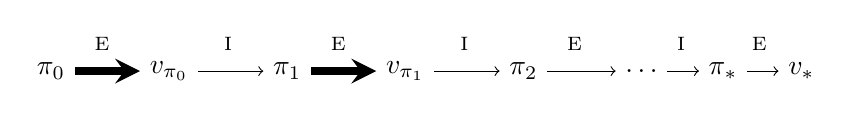
\begin{tikzpicture}
    \foreach \x in {0, 1, 2} {
      \node (p\x) at (\x * 3, 0) {$\pi_\x$};
      \node (e\x) at (\x * 3 + 0.65, 0.35) {\scriptsize E};
    }
    \foreach \x in {0, 1} {
      \node (v\x) at (\x * 3 + 1.5, 0) {$v_{\pi_\x}$};
      \draw[-stealth, line width=1mm] (p\x) -- (v\x);
    }
    \draw[->] (v0) -- (p1);
    \draw[->] (v1) -- (p2);
    \node at (2.25, 0.35) {\scriptsize I};
    \node at (5.25, 0.35) {\scriptsize I};
    \node (dots) at (3*2 + 1.5,  0) {$\ldots$};
    \draw[->] (p2) -- (dots);
    \node[right = 4mm of dots] (pistar) {$\pi_*$};
    \draw[->] (dots) -- (pistar);
    \node[right = 9.6mm of e2] (finali) {\scriptsize I};
    \node[right = 4mm of pistar] (vstar) {$v_*$};
    \draw[->] (pistar) -- (vstar);
    \node[right = 6mm of finali] {\scriptsize E};
  \end{tikzpicture}
\end{document}